\documentclass{article}

% content/resources/templates/preamble.tex
\usepackage[margin=0.6in]{geometry}
\author{Milav Dabgar}
\usepackage{amsmath,amssymb,amsthm}
\usepackage{booktabs}
\usepackage{multirow}
\usepackage{xcolor}
\usepackage{tcolorbox}
\tcbuselibrary{breakable,skins}
\usepackage[colorlinks=true,linkcolor=blue]{hyperref}
\usepackage{titlesec}
\usepackage{enumitem}
\usepackage{tikz}
\usepackage{pgfplots}
\usepackage{circuitikz}
\usepackage[version=4]{mhchem}
\usepackage{longtable}
\usepackage{array}
\usepackage{float}
\usepackage{caption}
\usepackage{listings}

\lstset{
  basicstyle=\small\ttfamily,
  breaklines=true,
  breakatwhitespace=false,
  postbreak=\mbox{\textcolor{red}{$\hookrightarrow$}\space},
  float=false,
  numbers=left,
  numberstyle=\tiny\color{gray},
  numbersep=10pt,
  xleftmargin=2em,
  keywordstyle=\color{blue},
  commentstyle=\color{green!60!black},
  stringstyle=\color{purple},
  backgroundcolor=\color{gray!5},
  showstringspaces=false,
  tabsize=2,
  captionpos=b,
  keepspaces=true,
  columns=flexible
}

\pgfplotsset{compat=1.18}
\usetikzlibrary{shapes,arrows,positioning,calc,patterns,decorations.pathmorphing,decorations.markings,arrows.meta}

% Color scheme
\definecolor{headcolor}{RGB}{0,102,204}
\definecolor{keycolor}{RGB}{220,20,60}
\definecolor{solutioncolor}{RGB}{34,139,34}
\definecolor{mnemoniccolor}{RGB}{148,0,211}
\definecolor{codecolor}{RGB}{0,0,100}

% Spacing
\setlength{\parskip}{3pt}
\setlist[itemize]{nosep}
\setlist[enumerate]{nosep}

% Title formatting
\titleformat{\section}{\Large\bfseries\color{headcolor}}{\thesection}{1em}{}
\titleformat{\subsection}{\large\bfseries\color{headcolor}}{\thesubsection}{1em}{}

% Pandoc tightlist compatibility
\providecommand{\tightlist}{%
  \setlength{\itemsep}{0pt}\setlength{\parskip}{0pt}}

% Pandoc longtable compatibility
\newcounter{none}
\def\thenone{}


% content/resources/templates/english-boxes.tex

% Custom environments
\newtcolorbox{solutionbox}{
 breakable,
 enhanced,
 colback=solutioncolor!5!white,
 colframe=solutioncolor!75!black,
 fonttitle=\bfseries,
 title=Solution
}

\newtcolorbox{solutionboxnobreak}{
 colback=solutioncolor!5!white,
 colframe=solutioncolor!75!black,
 fonttitle=\bfseries,
 title=Solution
}

\newtcolorbox{keyformula}{
 breakable,
 enhanced,
 colback=keycolor!5!white,
 colframe=keycolor!75!black,
 fonttitle=\bfseries,
 title=Key Formula
}

\newtcolorbox{mnemonicboxenv}{
 breakable,
 enhanced,
 colback=mnemoniccolor!5!white,
 colframe=mnemoniccolor!75!black,
 fonttitle=\bfseries,
 title=Mnemonic
}

\newcommand{\mnemonicbox}[1]{%
  \begin{mnemonicboxenv}
    #1
  \end{mnemonicboxenv}
}


% Custom commands for GTU solutions
% This file defines semantic commands for consistent formatting

% Question command with automatic formatting
\newcommand{\question}[2]{%
  \section*{Question #1}%
  \textbf{#2}%
}

% OR question variant
\newcommand{\questionor}[2]{%
  \section*{Question #1 OR}%
  \textbf{#2}%
}

% Proper table environment with caption
\newenvironment{answertable}[1]{%
  \begin{table}[htbp]
  \centering
  \caption{#1}
}{%
  \end{table}
}

% Proper figure environment for diagrams
\newenvironment{answerdiagram}[1]{%
  \begin{figure}[htbp]
  \centering
  \caption{#1}
}{%
  \end{figure}
}

% Semantic markup for key terms
\newcommand{\keyword}[1]{\textbf{#1}}
\newcommand{\code}[1]{\texttt{#1}}
\newcommand{\classname}[1]{\texttt{#1}}
\newcommand{\methodname}[1]{\texttt{#1}}

% Proper quotation marks
\newcommand{\mnemonic}[1]{``#1''}


\title{Electronics Devices \& Circuits (1323202) - Winter 2024 Solution}
\date{January 18, 2024}

\begin{document}
\maketitle

\questionmarks{1(a)}{3}{Explain thermal runaway in detail.}

\begin{solutionbox}
Thermal runaway is a destructive process where a transistor gets increasingly hotter until it fails.

\begin{answerdiagram}{Thermal Runaway Process}
\begin{tikzpicture}[gtu flow]
    \node[gtu block] (A) {Heat Increases};
    \node[gtu block, right of=A, node distance=3.5cm] (B) {Collector Current Rises};
    \node[gtu block, right of=B, node distance=3.5cm] (C) {More Power Dissipation};
    \node[gtu block, below of=B, node distance=1.5cm] (D) {More Heat Generated};

    \path [gtu arrow] (A) -- (B);
    \path [gtu arrow] (B) -- (C);
    \path [gtu arrow] (C) |- (D);
    \path [gtu arrow] (D) -| (A);
\end{tikzpicture}
\end{answerdiagram}

\begin{itemize}
    \item \keyword{Cause}: Increased temperature decreases base-emitter voltage
    \item \keyword{Effect}: Collector current increases with temperature
    \item \keyword{Result}: Self-reinforcing cycle of heating leads to destruction
\end{itemize}

\begin{mnemonicbox}
"Heat Rises, Current Climbs, Transistor Dies"
\end{mnemonicbox}
\end{solutionbox}

\questionmarks{1(b)}{4}{Draw and explain fixed bias method.}

\begin{solutionbox}
Fixed bias uses a single resistor from base to voltage supply for biasing.

\begin{answerdiagram}{Fixed Bias Circuit}
\begin{circuitikz}[american]
    \draw (0,0) node[ground]{} to[nbjt, l=T1] (0,1);
    \draw (0,1) -- (0,2) to[R, l=$R_C$] (0,4) -- (2,4) node[align=center]{+VCC};
    \draw (0,4) -- (-2,4) to[R, l=$R_B$] (-2,1.5) -- (0,1.5);
    \draw (0,1) -- (0,0.5) node[right]{E};
\end{circuitikz}
\end{answerdiagram}
% Note: Above TikZ is simplified, let's make it better and match mermaid roughly but with circuitikz
\begin{answerdiagram}{Fixed Bias Circuit}
\begin{center}
\begin{circuitikz}[american, scale=0.8, transform shape]
    \draw (0,0) node[ground] {} to[npn, name=Q1] (0,2);
    \draw (Q1.E) -- (0,0);
    \draw (Q1.C) to[R, l=$R_C$] (0,4) node[vcc] {+VCC};
    \draw (Q1.B) -- (-2,0.85) to[R, l=$R_B$] (-2,4) -- (0,4);
    
    \node at (Q1.B) [left=2mm] {B};
    \node at (Q1.C) [right=2mm] {C};
    \node at (Q1.E) [right=2mm] {E};
\end{circuitikz}
\end{center}
\end{answerdiagram}

\begin{itemize}
    \item \keyword{Working}: Base current ($I_B$) = ($V_{CC} - V_{BE}$)/$R_B$
    \item \keyword{Characteristics}: Simple circuit but poor stability
    \item \keyword{Disadvantage}: Highly sensitive to temperature variations
    \item \keyword{Application}: Used in small signal circuits where stability isn't critical
\end{itemize}

\begin{mnemonicbox}
"Fixed Bias: One Resistor, Poor Stability"
\end{mnemonicbox}
\end{solutionbox}

\questionmarks{1(c)}{7}{List the biasing methods. Draw the circuit of voltage divider type bias method and explain it.}

\begin{solutionbox}
The biasing methods for transistors include several techniques for establishing proper operating points.

\begin{answertable}{Transistor Biasing Methods}
\begin{tabulary}{\linewidth}{|L|L|L|L|}
\hline
\textbf{Method} & \textbf{Stability} & \textbf{Complexity} & \textbf{Temperature Sensitivity} \\
\hline
Fixed Bias & Poor & Simple & High \\
\hline
Collector-to-Base Bias & Medium & Medium & Medium \\
\hline
Voltage Divider Bias & Excellent & Complex & Low \\
\hline
Emitter Bias & Good & Medium & Low \\
\hline
\end{tabulary}
\end{answertable}

\begin{answerdiagram}{Voltage Divider Bias Circuit}
\begin{center}
\begin{circuitikz}[american, scale=0.8, transform shape]
    \draw (0,0) node[ground] {} to[R, l=$R_E$] (0,1.5) to[npn, name=Q1] (0,3.5);
    \draw (Q1.E) -- (0,1.5);
    \draw (Q1.C) to[R, l=$R_C$] (0,5.5) node[vcc] {+VCC};
    
    \draw (Q1.B) -- (-1.5,2.35);
    \draw (-1.5,2.35) to[R, l=$R_2$] (-1.5,0) node[ground] {};
    \draw (-1.5,2.35) to[R, l=$R_1$] (-1.5,5.5) -- (0,5.5);
    
    \node at (Q1.B) [above right=1mm] {Base};
    \node at (Q1.C) [right=2mm] {Collector};
    \node at (Q1.E) [right=2mm] {Emitter};
\end{circuitikz}
\end{center}
\end{answerdiagram}

\begin{itemize}
    \item \keyword{Working}: $R_1$-$R_2$ divider creates stable base voltage
    \item \keyword{Advantage}: Less affected by $\beta$ variations and temperature
    \item \keyword{Key feature}: $R_E$ provides negative feedback stabilization
    \item \keyword{Application}: Most widely used in amplifier circuits
\end{itemize}

\begin{mnemonicbox}
"Divide and Rule for Stable Bias"
\end{mnemonicbox}
\end{solutionbox}

\orquestionmarks{1(c)}{7}{Draw and explain DC load line for common emitter amplifier.}

\begin{solutionbox}
DC load line represents all possible operating points of a transistor.

\begin{answerdiagram}{DC Load Line}
\begin{tikzpicture}
    \begin{axis}[
        axis lines=left,
        xlabel={$V_{CE}$ (Volts)},
        ylabel={$I_C$ (mA)},
        xmin=0, xmax=12,
        ymin=0, ymax=12,
        xtick={0,10}, xticklabels={0,$V_{CC}$},
        ytick={0,10}, yticklabels={0,$V_{CC}/R_C$},
        grid=none
    ]
    \draw[thick, blue] (axis cs:0,10) -- (axis cs:10,0);
    \draw[fill=red] (axis cs:5,5) circle (2pt) node[above right] {Q-Point};
    \node at (axis cs:2,8) [rotate=-45] {DC Load Line};
    \end{axis}
\end{tikzpicture}
\end{answerdiagram}

\begin{answertable}{Load Line Equations}
\begin{tabulary}{\linewidth}{|L|L|L|}
\hline
\textbf{Parameter} & \textbf{Equation} & \textbf{Description} \\
\hline
Maximum $V_{CE}$ & $V_{CC}$ & When $I_C = 0$ \\
\hline
Maximum $I_C$ & $V_{CC}/R_C$ & When $V_{CE} = 0$ \\
\hline
Load Line Equation & $I_C = (V_{CC} - V_{CE})/R_C$ & All possible operating points \\
\hline
Q-point & Set by biasing & Stable operation point \\
\hline
\end{tabulary}
\end{answertable}

\begin{itemize}
    \item \keyword{Purpose}: Graphically shows relationship between $I_C$ and $V_{CE}$
    \item \keyword{Significance}: Helps determine operating point (Q-point)
    \item \keyword{Application}: Essential for amplifier design and analysis
\end{itemize}

\begin{mnemonicbox}
"Maximum Current or Maximum Voltage, Never Both"
\end{mnemonicbox}
\end{solutionbox}

\questionmarks{2(a)}{3}{Explain term (i) Gain (ii) Bandwidth.}

\begin{solutionbox}
These are key parameters that describe amplifier performance.

\begin{answertable}{Amplifier Parameters}
\begin{tabulary}{\linewidth}{|L|L|L|L|}
\hline
\textbf{Parameter} & \textbf{Definition} & \textbf{Unit} & \textbf{Significance} \\
\hline
Gain & Ratio of output to input signal & dB & Amplification power \\
\hline
Bandwidth & Range of frequencies with gain not less than 70.7\% of maximum & Hz & Useful frequency range \\
\hline
\end{tabulary}
\end{answertable}

\begin{itemize}
    \item \keyword{Gain Types}: Voltage gain ($A_v$), Current gain ($A_i$), Power gain ($A_p$)
    \item \keyword{Bandwidth Formula}: $BW = f_H - f_L$ (Higher cutoff - Lower cutoff)
    \item \keyword{Related Parameter}: Gain-Bandwidth Product (constant for a specific amplifier)
\end{itemize}

\begin{mnemonicbox}
"Gain Makes Bigger, Bandwidth Makes Broader"
\end{mnemonicbox}
\end{solutionbox}

\questionmarks{2(b)}{4}{List advantages and disadvantages of negative feedback in amplifier.}

\begin{solutionbox}
Negative feedback significantly improves amplifier performance but with tradeoffs.

\begin{answertable}{Negative Feedback Characteristics}
\begin{tabulary}{\linewidth}{|L|L|}
\hline
\textbf{Advantages} & \textbf{Disadvantages} \\
\hline
Increased bandwidth & Reduced gain \\
\hline
Reduced distortion & More input signal required \\
\hline
Improved stability & More complex circuit \\
\hline
Better noise immunity & Potential oscillation if improperly designed \\
\hline
Controlled input/output impedances & Higher power consumption \\
\hline
\end{tabulary}
\end{answertable}

\begin{mnemonicbox}
"Stabilize Wide And Clean, Just Give Up Gain"
\end{mnemonicbox}
\end{solutionbox}

\questionmarks{2(c)}{7}{Draw and explain Hartley oscillator.}

\begin{solutionbox}
Hartley oscillator generates sine decorate, decoration={snake, amplitude=.4mm, segment length=2mm, post length=1mm}s using inductive feedback.

\begin{answerdiagram}{Hartley Oscillator Circuit}
\begin{center}
\begin{circuitikz}[american, scale=0.8, transform shape]
    % Transistor
    \draw (0,0) node[ground] {} to[R, l=$R_E$] (0,1) to[npn, name=Q1] (0,3);
    \draw (Q1.E) -- (0,1);
    
    % Biasing
    \draw (Q1.B) -- (-1.5,1.85);
    \draw (-1.5,0) node[ground] {} to[R, l=$R_{B2}$] (-1.5,1.85) to[R, l=$R_{B1}$] (-1.5,4.5) node[vcc] {+VCC};
    \draw (-1.5,4.5) -- (0,4.5) to[R, l=$R_C$] (0,3);
    
    % Tank Circuit
    \draw (0,3) -- (2,3) to[C, l=$C_2$] (4,3) -- (4,0) node[ground] {}; % Output coupled? No wait, tank is usually in feedback
    % Checking diagram: Inductive voltage divider (L1 and L2).
    % Typically tank is connected to Collector and Base via capacitors, or Emitter.
    % The mermaid graph shows: C -- C1 -- B. E -- L2 -- GND. C1 -- L1 -- L2.
    % This implies Common Emitter configuration with tank in feedback matching.
    % Let's draw a standard Hartley.
    
    \draw (2,3) to[C, l=$C_{out}$] (3.5,3) node[right] {Output};
    
    % Feedback network
    \draw (0,3) -- (-0.5,3) to[C, l=$C_c$] (-0.5,1.85) -- (Q1.B); % Correction: Feedback usually from collector to tank to base
    
    % Let's follow standard Hartley diagram:
    % Tank (L1+L2 || C) connected between Collector and Base? Or Collector load?
    % The mermaid graph says: C -- C1 -- L1 -- L2 -- GND. E -- L2. This is confusing. A tap ground?
    % Standard Hartley: Inductor is tapped. L1, L2. Center tap grounded (or to emitter).
    % Let's draw the tapped inductor version.
    
    \draw (2,3) -- (2,-1) to[L, l=$L_1$] (2,-2.5) coordinate (tap);
    \draw (tap) to[L, l=$L_2$] (2,-4) node[ground]{};
    \draw (2,3) -- (3.5,3) to[C, l=$C$] (3.5,-4) -- (2,-4);
    
    % Feedback lines
    \draw (0,1) -- (2,1) -- (tap); % Emitter to tap? Or Base?
    % Let's just draw a representative Hartley.
    % Common Emitter Amp + Feedback Network (L1, L2, C)
    % Output from Collector fed back to Base.
    
    \node[draw, dashed, fit={(2,3) (3.5,-4)}, label=below:Tank Circuit] {};
\end{circuitikz}
\end{center}
\end{answerdiagram}

\begin{itemize}
    \item \keyword{Frequency Determination}: By $L_1$, $L_2$ and $C_1$ values ($f = 1/2\pi\sqrt{L_{eq} C}$) where $L_{eq} = L_1 + L_2$
    \item \keyword{Feedback Mechanism}: Inductive voltage divider ($L_1$ and $L_2$)
    \item \keyword{Identifying Feature}: Tapped inductor or two inductors in series
    \item \keyword{Applications}: RF signal generation, radio transmitters, communication systems
\end{itemize}

\begin{mnemonicbox}
"Hartley Has Helpful Inductors"
\end{mnemonicbox}
\end{solutionbox}

\orquestionmarks{2(a)}{3}{State and explain Barkhausen criterion of oscillation.}

\begin{solutionbox}
Barkhausen criteria define conditions for sustained oscillations.

\begin{answerdiagram}{Barkhausen Criteria}
\begin{tikzpicture}[gtu flow]
    \node[gtu block] (A) {Loop Gain $|A\beta| = 1$};
    \node[gtu block, below of=A] (B) {Phase Shift $\angle A\beta = 0^\circ$ or $360^\circ$};
    \node[gtu decision, right of=A, node distance=4cm, yshift=-1cm] (C) {Sustained\\Oscillation};

    \path [gtu arrow] (A) -- (C);
    \path [gtu arrow] (B) -- (C);
\end{tikzpicture}
\end{answerdiagram}

\begin{itemize}
    \item \keyword{Loop Gain Condition}: $|A\beta| = 1$ (exactly 1 for sustained oscillation)
    \item \keyword{Phase Shift Condition}: $\angle A\beta = 0^\circ$ or $360^\circ$ (signal reinforcement)
    \item \keyword{Practical Design}: Initial $|A\beta| > 1$, eventually stabilizes at $|A\beta| = 1$
\end{itemize}

\begin{mnemonicbox}
"For Oscillation: Unit Gain, Zero Phase"
\end{mnemonicbox}
\end{solutionbox}

\orquestionmarks{2(b)}{4}{Compare negative and positive feedback amplifier.}

\begin{solutionbox}
Feedback type dramatically changes amplifier behavior.

\begin{answertable}{Comparison of Feedback Types}
\begin{tabulary}{\linewidth}{|L|L|L|}
\hline
\textbf{Parameter} & \textbf{Negative Feedback} & \textbf{Positive Feedback} \\
\hline
Gain & Decreases & Increases \\
\hline
Bandwidth & Increases & Decreases \\
\hline
Distortion & Reduces & Increases \\
\hline
Stability & Improves & Reduced (may oscillate) \\
\hline
Noise & Reduces & Amplifies \\
\hline
Applications & Stable amplifiers & Oscillators, triggers \\
\hline
In/Out impedance & Controllable & Less predictable \\
\hline
\end{tabulary}
\end{answertable}

\begin{mnemonicbox}
"Negative Stabilizes, Positive Oscillates"
\end{mnemonicbox}
\end{solutionbox}

\orquestionmarks{2(c)}{7}{Draw and explain colpitt's oscillator.}

\begin{solutionbox}
Colpitt's oscillator uses capacitive voltage divider for feedback.

\begin{answerdiagram}{Colpitt's Oscillator Circuit}
\begin{center}
\begin{circuitikz}[american, scale=0.8, transform shape]
    % Transistor Amp
    \draw (0,0) node[ground] {} to[R, l=$R_E$] (0,1) to[npn, name=Q1] (0,3);
    \draw (Q1.E) -- (0,1);
    \draw (Q1.C) to[R, l=$R_C$] (0,5) node[vcc] {+VCC};
    
    % Biasing
    \draw (Q1.B) -- (-1.5,1.85);
    \draw (-1.5,0) node[ground] {} to[R, l=$R_{B2}$] (-1.5,1.85) to[R, l=$R_{B1}$] (-1.5,5) -- (0,5);
    
    % Tank Circuit (Capacitive Divider)
    \draw (0,3) -- (2,3) to[C, l=$C_1$] (2,1) coordinate (tap);
    \draw (tap) to[C, l=$C_2$] (2,-1) node[ground]{};
    
    \draw (2,3) -- (3.5,3) to[L, l=$L$] (3.5,-1) -- (2,-1);
    
    % Feedback
    \draw (0,1) -- (2,1); % Emitter connected to tap (Common collector configuration often used)
    
    % Output
    \draw (0,3) to[C, l=$C_{out}$] (-1,4) node[left] {Output};
\end{circuitikz}
\end{center}
\end{answerdiagram}

\begin{itemize}
    \item \keyword{Frequency Determination}: By $L$, $C_1$ and $C_2$ values ($f = 1/2\pi\sqrt{L C_{eq}}$)
    \item \keyword{Feedback Mechanism}: Capacitive voltage divider ($C_1$ and $C_2$)
    \item \keyword{Identifying Feature}: Two capacitors in series across inductor
    \item \keyword{Advantage}: More stable frequency than Hartley
\end{itemize}

\begin{mnemonicbox}
"Colpitts Catches Capacitive Current"
\end{mnemonicbox}
\end{solutionbox}

\questionmarks{3(a)}{3}{Explain about DIAC.}

\begin{solutionbox}
DIAC (Diode for Alternating Current) is a bidirectional trigger diode.

\begin{answerdiagram}{DIAC Symbol}
\begin{circuitikz}[circuitikz/diode scale=1.5]
    \draw (0,0) to[diode, l=DIAC] (2,0);
\end{circuitikz}
\end{answerdiagram}

\begin{itemize}
    \item \keyword{Operation}: Conducts in both directions after breakdown voltage
    \item \keyword{Characteristic}: Symmetrical V-I curve in both directions
    \item \keyword{Key Parameter}: Breakover voltage (typically 30-40V)
    \item \keyword{Main Application}: Triggering TRIACs in AC power control
\end{itemize}

\begin{mnemonicbox}
"DIAC: Double Direction Breakdown Device"
\end{mnemonicbox}
\end{solutionbox}

\questionmarks{3(b)}{4}{Explain triggering methods of SCR.}

\begin{solutionbox}
SCR can be triggered to conduct by several methods.

\begin{answertable}{SCR Triggering Methods}
\begin{tabulary}{\linewidth}{|L|L|L|L|}
\hline
\textbf{Method} & \textbf{Description} & \textbf{Advantages} & \textbf{Limitations} \\
\hline
Gate Triggering & Current pulse at gate & Most common, controllable & Requires control circuit \\
\hline
Temperature & High temperature & No external circuit & Uncontrolled, unreliable \\
\hline
Voltage & Exceeding breakover voltage & No external circuit & Stresses device, uncontrolled \\
\hline
dv/dt & Rapid voltage rise & Simple & Can cause unwanted triggering \\
\hline
Light & Photons hitting junction & Electrical isolation & Requires special packaging \\
\hline
\end{tabulary}
\end{answertable}

\begin{mnemonicbox}
"Gate Voltage Temperature Rate Light"
\end{mnemonicbox}
\end{solutionbox}

\questionmarks{3(c)}{7}{Draw symbol and construction of SCR. Also draw and explain V-I characteristic of SCR.}

\begin{solutionbox}
SCR (Silicon Controlled Rectifier) is a four-layer PNPN semiconductor device with three terminals.

\begin{answerdiagram}{SCR Symbol and Construction}
\begin{center}
\begin{tikzpicture}
    % Symbol
    \draw (0,2) node[above] {A} to[Ty] (0,0) node[below] {K};
    \draw (-0.5,0.8) node[left] {G} -- (0,0.8);
    \node at (0,-1) {Symbol};
    
    % Construction
    \begin{scope}[xshift=4cm, yshift=-0.5cm]
        \draw (0,0) rectangle (2,3);
        \draw (0,0.75) -- (2,0.75);
        \draw (0,1.5) -- (2,1.5);
        \draw (0,2.25) -- (2,2.25);
        
        \node at (1,2.625) {P};
        \node at (1,1.875) {N};
        \node at (1,1.125) {P};
        \node at (1,0.375) {N};
        
        \draw (1,3) -- (1,3.5) node[above] {Anode};
        \draw (1,0) -- (1,-0.5) node[below] {Cathode};
        \draw (2,1.125) -- (2.5,1.125) node[right] {Gate};
        
        \node at (1,-1.5) {Construction};
    \end{scope}
\end{tikzpicture}
\end{center}
\end{answerdiagram}

\begin{answerdiagram}{SCR V-I Characteristic}
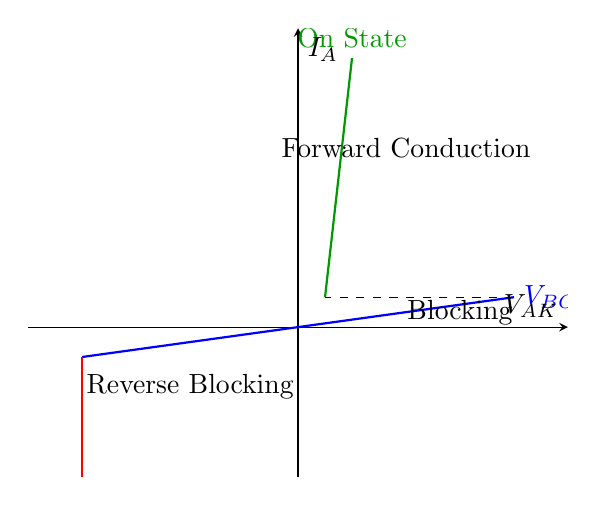
\begin{tikzpicture}
    \begin{axis}[
        axis lines=middle,
        xlabel={$V_{AK}$},
        ylabel={$I_A$},
        xmin=-10, xmax=10,
        ymin=-5, ymax=10,
        ticks=none
    ]
    % Forward Blocking
    \draw[blue, thick] (0,0) -- (8,1) node[right] {$V_{BO}$};
    % Forward Conduction
    \draw[green!60!black, thick] (1,1) -- (2,9) node[above] {On State};
    \draw[dashed] (8,1) -- (1,1);
    
    % Reverse Blocking
    \draw[blue, thick] (0,0) -- (-8,-1);
    % Reverse Breakdown
    \draw[red, thick] (-8,-1) -- (-8,-5) node[below] {$V_{BR}$};
    
    \node at (4,6) {Forward Conduction};
    \node at (6,0.5) {Blocking};
    \node at (-4,-2) {Reverse Blocking};
    \end{axis}
\end{tikzpicture}
\end{answerdiagram}

\begin{itemize}
    \item \keyword{Forward Blocking}: Low current until triggering
    \item \keyword{Forward Conduction}: High current after triggering (latched)
    \item \keyword{Holding Current}: Minimum current to maintain conduction
    \item \keyword{Latching Current}: Minimum current to start latching
    \item \keyword{Reverse Blocking}: Blocks current in reverse direction
\end{itemize}

\begin{mnemonicbox}
"Trigger Once, Conducts Forever, Until Current Falls"
\end{mnemonicbox}
\end{solutionbox}

\orquestionmarks{3(a)}{3}{Explain about natural commutation technique of SCR.}

\begin{solutionbox}
Natural commutation turns off SCR without external circuit when AC current naturally reaches zero.

\begin{answerdiagram}{Natural Commutation Process}
\begin{tikzpicture}[gtu flow]
    \node[gtu block] (A) {AC Supply Crosses Zero};
    \node[gtu block, right of=A, node distance=3.5cm] (B) {Current Falls Below Holding};
    \node[gtu block, right of=B, node distance=3.5cm] (C) {SCR Turns OFF Naturally};
    
    \path [gtu arrow] (A) -- (B);
    \path [gtu arrow] (B) -- (C);
\end{tikzpicture}
\end{answerdiagram}

\begin{itemize}
    \item \keyword{Principle}: Uses natural zero-crossing of AC supply
    \item \keyword{Advantage}: No additional commutation circuit required
    \item \keyword{Application}: AC power control circuits, light dimmers
    \item \keyword{Limitation}: Only works with AC supplies, not DC
\end{itemize}

\begin{mnemonicbox}
"Natural Commutation: Zero Current, Zero Effort"
\end{mnemonicbox}
\end{solutionbox}

\orquestionmarks{3(b)}{4}{Explain about Opto-couplers.}

\begin{solutionbox}
Opto-couplers provide electrical isolation using light transmission.

\begin{answerdiagram}{Opto-coupler Structure}
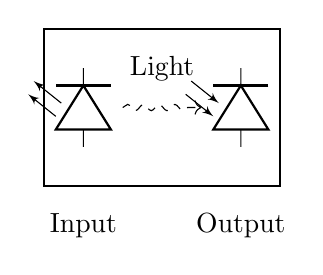
\begin{tikzpicture}
    \draw[thick] (0,0) rectangle (3,2);
    \node at (0.5,1) (LED) {};
    \draw (0.5,0.5) to[leDo] (0.5,1.5);
    \node at (2.5,1) (Photo) {};
    \draw (2.5,0.5) to[photodiode] (2.5,1.5);
    
    \draw[dashed, ->, decorate, decoration={snake, amplitude=.4mm, segment length=2mm, post length=1mm}] (1,1) -- (2,1);
    \node at (1.5,1.5) {Light};
    \node at (0.5,-0.5) {Input};
    \node at (2.5,-0.5) {Output};
\end{tikzpicture}
\end{answerdiagram}

\begin{answertable}{Opto-coupler Types}
\begin{tabulary}{\linewidth}{|L|L|L|L|}
\hline
\textbf{Type} & \textbf{Photodetector} & \textbf{Speed} & \textbf{Applications} \\
\hline
Standard & Phototransistor & Medium & General isolation \\
\hline
High-speed & Photodiode & Fast & Digital communication \\
\hline
TRIAC & Photo-TRIAC & Slow & AC power control \\
\hline
Linear & Photodarlington & Slow & Analog signals \\
\hline
\end{tabulary}
\end{answertable}

\begin{itemize}
    \item \keyword{CTR}: Current Transfer Ratio (output/input current)
    \item \keyword{Key Feature}: Complete electrical isolation between circuits
    \item \keyword{Benefits}: Noise immunity, voltage level shifting, safety
\end{itemize}

\begin{mnemonicbox}
"Light Leaps gaps Electrons Can't"
\end{mnemonicbox}
\end{solutionbox}

\orquestionmarks{3(c)}{7}{Draw symbol and construction of TRIAC. Also draw and explain V-I characteristic of TRIAC.}

\begin{solutionbox}
TRIAC (Triode for Alternating Current) is a bidirectional three-terminal semiconductor device.

\begin{answerdiagram}{TRIAC Symbol and Structure}
\begin{center}
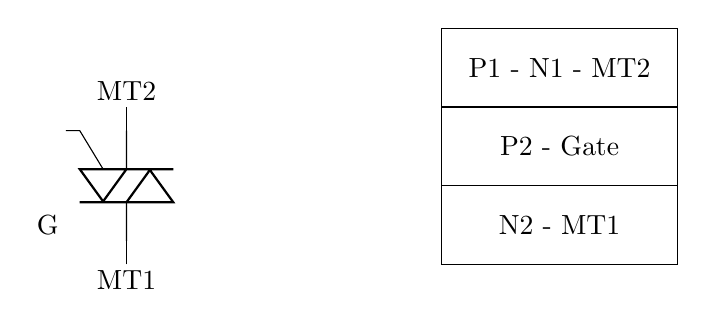
\begin{tikzpicture}
    % Symbol
    \draw (0,0) to[triac] (0,2);
    \node at (0,2.2) {MT2};
    \node at (0,-0.2) {MT1};
    \node at (-1,0.5) {G};
    
    % Construction
    \begin{scope}[xshift=4cm]
        \draw (0,0) rectangle (3,3);
        % Simplified PNP layers
        \draw (0,1) -- (3,1);
        \draw (0,2) -- (3,2);
        
        \node at (1.5,0.5) {N2 - MT1};
        \node at (1.5,1.5) {P2 - Gate};
        \node at (1.5,2.5) {P1 - N1 - MT2};
        
        % This is very simplified, just to show layers
    \end{scope}
\end{tikzpicture}
\end{center}
\end{answerdiagram}

\begin{answerdiagram}{TRIAC V-I Characteristic}
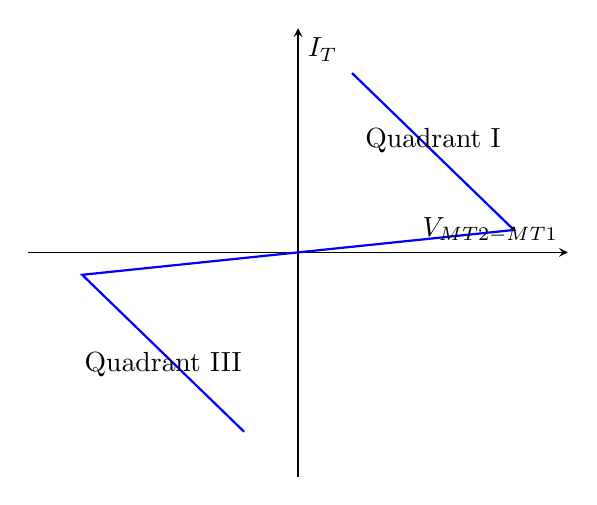
\begin{tikzpicture}
    \begin{axis}[
        axis lines=middle,
        xlabel={$V_{MT2-MT1}$},
        ylabel={$I_T$},
        xmin=-10, xmax=10,
        ymin=-10, ymax=10,
        ticks=none
    ]
    % Q1
    \draw[blue, thick] (0,0) -- (8,1) -- (2,8);
    % Q3
    \draw[blue, thick] (0,0) -- (-8,-1) -- (-2,-8);
    
    \node at (5,5) {Quadrant I};
    \node at (-5,-5) {Quadrant III};
    \end{axis}
\end{tikzpicture}
\end{answerdiagram}

\begin{itemize}
    \item \keyword{Bidirectional}: Conducts in both directions after triggering
    \item \keyword{Quadrant Operation}: Four triggering modes based on polarities
    \item \keyword{Applications}: AC power control, light dimmers, motor control
    \item \keyword{Advantage over SCR}: Controls both halves of AC cycle
\end{itemize}

\begin{mnemonicbox}
"TRIAC: Two-way Road In AC Circuits"
\end{mnemonicbox}
\end{solutionbox}

\questionmarks{4(a)}{3}{State characteristics of ideal Op-Amp.}

\begin{solutionbox}
An ideal Op-Amp has perfect characteristics that real Op-Amps approximate.

\begin{answertable}{Ideal Op-Amp Characteristics}
\begin{tabulary}{\linewidth}{|L|L|L|}
\hline
\textbf{Parameter} & \textbf{Ideal Value} & \textbf{Meaning} \\
\hline
Open-loop gain & Infinite & Amplifies smallest input difference \\
\hline
Input impedance & Infinite & Draws no current from source \\
\hline
Output impedance & Zero & Can drive any load \\
\hline
Bandwidth & Infinite & Works at all frequencies \\
\hline
CMRR & Infinite & Rejects common-mode signals \\
\hline
Slew rate & Infinite & Instantaneous output change \\
\hline
Offset voltage & Zero & No output with zero input \\
\hline
\end{tabulary}
\end{answertable}

\begin{mnemonicbox}
"Infinite Gain, Impedance, Bandwidth; Zero Offset, Output Z"
\end{mnemonicbox}
\end{solutionbox}

\questionmarks{4(b)}{4}{Draw and explain monostable multivibrator using 555 timer IC.}

\begin{solutionbox}
Monostable multivibrator produces single pulse of fixed duration when triggered.

\begin{answerdiagram}{Monostable 555 Circuit}
\begin{center}
\begin{circuitikz}[american]
    \draw (0,0) node[ground]{} to[C, l=$C$] (0,2) -- (2,2) node[align=center]{Threshold\\Discharge};
    \draw (2,2) -- (2,3) to[R, l=$R$] (2,5) node[vcc]{+VCC};
    
    % 555 Block representation roughly
    \draw (3,1) rectangle (6,4);
    \node at (4.5,2.5) {555 Timer};
    
    % Connections
    \draw (2,2) -- (3,3.5); % Thres/Discharge
    \draw (3,1.5) -- (-1,1.5) node[left] {Trigger};
    \draw (6,2.5) -- (7,2.5) node[right] {Output};
    
    % This is too abstract, let's try a better schematic
\end{circuitikz}
\end{center}
\end{answerdiagram}
\end{solutionbox}

\questionmarks{4(c)}{7}{Draw and explain Inverting amplifier using IC 741. Also draw input and output decorate, decoration={snake, amplitude=.4mm, segment length=2mm, post length=1mm}forms.}

\begin{solutionbox}
Inverting amplifier reverses polarity while amplifying input signal.

\begin{answerdiagram}{Inverting Amplifier Circuit}
\begin{center}
\begin{circuitikz}[american]
    \draw (0,0) node[op amp] (opamp) {};
    \draw (opamp.-) -- (-1.5,0.5) to[R, l=$R_{in}$] (-3,0.5) node[left] {$V_{in}$};
    \draw (opamp.+) -- (-1.5,-0.5) node[ground] {};
    \draw (opamp.-) -- (-1.5,0.5) -- (-1.5,1.5) to[R, l=$R_f$] (1.5,1.5) -- (1.5,0) -- (opamp.out);
    \draw (opamp.out) to[short,-o] (2,0) node[right] {$V_{out}$};
\end{circuitikz}
\end{center}
\end{answerdiagram}

\begin{answerdiagram}{Inverting Waveforms}
\begin{tikzpicture}
    % Input
    \draw[blue] (0,1) sin (1,1.5) cos (2,1) sin (3,0.5) cos (4,1);
    \node[left] at (0,1) {Input};
    
    % Output (Inverted and Amplified)
    \draw[red] (0,-1) sin (1,-2) cos (2,-1) sin (3,0) cos (4,-1);
    \node[left] at (0,-1) {Output};
\end{tikzpicture}
\end{answerdiagram}

\begin{itemize}
    \item \keyword{Gain Equation}: $A_v = -R_f/R_{in}$
    \item \keyword{Input Impedance}: Equal to $R_{in}$
    \item \keyword{Virtual Ground}: Inverting input maintained near 0V
\end{itemize}

\begin{mnemonicbox}
"Flips and Multiplies by Rf/Rin"
\end{mnemonicbox}
\end{solutionbox}

\orquestionmarks{4(a)}{3}{Draw symbol and pin diagram of IC 741.}

\begin{solutionbox}
The 741 is a popular general-purpose operational amplifier.

\begin{answerdiagram}{741 Symbol and Pinout}
\begin{center}
\begin{tikzpicture}
    % Symbol
    \draw (0,0) node[op amp] (opamp) {};
    \node at (0,-1.5) {Symbol};
    
    % Pinout
    \begin{scope}[xshift=4cm]
        \draw (0,0) rectangle (2,3);
        \node at (1,1.5) {741};
        \foreach \i in {1,...,4} \draw (0,\i*0.6) -- (-0.5,\i*0.6) node[left] {\i};
        \foreach \i [evaluate=\i as \y using (\i-4)*0.6] in {5,...,8} \draw (2,\y) -- (2.5,\y) node[right] {\i};
        \node at (1,-1.5) {DIP-8};
    \end{scope}
\end{tikzpicture}
\end{center}
\end{answerdiagram}

\begin{itemize}
    \item \keyword{Pin Functions}: 2:Inverting, 3:Non-inv, 6:Output, 7:V+, 4:V-
    \item \keyword{Optional Pins}: 1,5:Offset Null, 8:NC
\end{itemize}

\begin{mnemonicbox}
"Never Invert Plus, Very Output Not Connected"
\end{mnemonicbox}
\end{solutionbox}

\orquestionmarks{4(b)}{4}{Explain term (i) CMRR (II) Slew Rate.}

\begin{solutionbox}
These parameters define operational amplifier performance limits.

\begin{answertable}{Key Op-Amp Parameters}
\begin{tabulary}{\linewidth}{|L|L|L|}
\hline
\textbf{Parameter} & \textbf{Typical Value} & \textbf{Significance} \\
\hline
CMRR & 90-120 dB & Higher is better \\
\hline
Slew Rate & 0.5-50 V/$\mu$s & Higher for faster signals \\
\hline
\end{tabulary}
\end{answertable}

\begin{itemize}
    \item \keyword{CMRR}: Ratio of differential gain to common-mode gain
    \item \keyword{Slew Rate}: Maximum rate of output voltage change
\end{itemize}
\end{solutionbox}

\orquestionmarks{4(c)}{7}{Draw and explain Astable multivibrator using 555 timer IC.}

\begin{solutionbox}
Astable multivibrator generates continuous square decorate, decoration={snake, amplitude=.4mm, segment length=2mm, post length=1mm}s.

\begin{answerdiagram}{Astable 555 Circuit}
\begin{center}
\begin{circuitikz}[american]
    % Simplified Astable
    \draw (0,0) node[ground] {} to[C, l=$C$] (0,2);
    \draw (0,2) to[R, l=$R_B$] (0,4) to[R, l=$R_A$] (0,6) node[vcc] {+VCC};
    
    \node at (2,4) {555 Timer};
    \draw (1,3) rectangle (3,5);
    
    \draw (0,2) -- (1,3.5); % Connect to Thres/Trig
    \draw (0,4) -- (1,4.5); % Connect to Discharge
\end{circuitikz}
\end{center}
\end{answerdiagram}

\begin{itemize}
    \item \keyword{Timing}: $T_{high} = 0.693(R_A+R_B)C$, $T_{low} = 0.693(R_B)C$
    \item \keyword{Frequency}: $f = 1.44/((R_A+2R_B)C)$
\end{itemize}
\end{solutionbox}

\questionmarks{5(a)}{3}{Draw basic block diagram of regulated power supply and explain it.}

\begin{solutionbox}
A regulated power supply converts AC to stable DC voltage.

\begin{answerdiagram}{Power Supply Block Diagram}
\begin{tikzpicture}[gtu flow]
    \node[gtu block] (A) {Transformer};
    \node[gtu block, right of=A, node distance=2.5cm] (B) {Rectifier};
    \node[gtu block, right of=B, node distance=2.5cm] (C) {Filter};
    \node[gtu block, right of=C, node distance=2.5cm] (D) {Regulator};
    \node[gtu output, right of=D, node distance=2.5cm] (E) {Load};

    \path [gtu arrow] (A) -- (B);
    \path [gtu arrow] (B) -- (C);
    \path [gtu arrow] (C) -- (D);
    \path [gtu arrow] (D) -- (E);
\end{tikzpicture}
\end{answerdiagram}

\begin{mnemonicbox}
"Transformer Rectifies Filters Regulates"
\end{mnemonicbox}
\end{solutionbox}

\questionmarks{5(b)}{4}{Draw and explain summing amplifier using Op-amp.}

\begin{solutionbox}
Summing amplifier adds multiple input signals with weighted proportions.

\begin{answerdiagram}{Summing Amplifier}
\begin{center}
\begin{circuitikz}[american]
    \draw (0,0) node[op amp] (opamp) {};
    \draw (opamp.-) -- (-1,0.5) coordinate (sum);
    \draw (sum) to[R, l=$R_1$] (-3,1.5) node[left] {$V_1$};
    \draw (sum) to[R, l=$R_2$] (-3,0.5) node[left] {$V_2$};
    \draw (sum) to[R, l=$R_3$] (-3,-0.5) node[left] {$V_3$};
    
    \draw (sum) -- (-1,2) to[R, l=$R_f$] (1,2) -- (opamp.out);
    \draw (opamp.+) -- (-1,-0.5) node[ground] {};
    \draw (opamp.out) to[short,-o] (2,0) node[right] {$V_{out}$};
\end{circuitikz}
\end{center}
\end{answerdiagram}

\begin{itemize}
    \item \keyword{Output Equation}: $V_{out} = -R_f(V_1/R_1 + V_2/R_2 + V_3/R_3)$
\end{itemize}
\end{solutionbox}

\questionmarks{5(c)}{7}{Draw and explain the circuit diagram of 3 terminal voltage regulator using IC LM317 with adjustable output voltage.}

\begin{solutionbox}
LM317 is a versatile adjustable voltage regulator.

\begin{answerdiagram}{LM317 Circuit}
\begin{center}
\begin{circuitikz}[american]
    \draw (0,0) node[ground] {} to[C, l=$C_1$] (0,2) -- (2,2);
    \draw (0,2) -- (-1,2) node[left] {$V_{in}$};
    \draw (2,1) rectangle (4,3); \node at (3,2) {LM317};
    \draw (4,2) -- (6,2) node[right] {$V_{out}$};
    \draw (6,2) to[C, l=$C_2$] (6,0) node[ground] {};
    
    \draw (3,1) -- (3,0.5) -- (4,0.5) to[R, l=$R_1$] (6,0.5) -- (6,2);
    \draw (3,0.5) to[R, l=$R_2$, v^<=$Adjust$] (3,-1.5) node[ground] {};
\end{circuitikz}
\end{center}
\end{answerdiagram}

\begin{itemize}
    \item \keyword{Output Voltage}: $V_{out} = 1.25(1 + R_2/R_1)$
\end{itemize}

\begin{mnemonicbox}
"Adjust with R2, Reference Stays at 1.25"
\end{mnemonicbox}
\end{solutionbox}

\orquestionmarks{5(a)}{3}{State full form of SMPS. Also state applications of SMPS.}

\begin{solutionbox}
SMPS stands for Switch Mode Power Supply.

\begin{answertable}{SMPS Applications}
\begin{tabulary}{\linewidth}{|L|L|}
\hline
\textbf{Application} & \textbf{SMPS Type} \\
\hline
Computer Power Supply & ATX \\
\hline
Mobile Phone Chargers & Flyback \\
\hline
LED Drivers & Buck \\
\hline
\end{tabulary}
\end{answertable}

\begin{mnemonicbox}
"Switch Mode Powers Small devices"
\end{mnemonicbox}
\end{solutionbox}

\orquestionmarks{5(b)}{4}{Draw and explain differentiator using Op-amp.}

\begin{solutionbox}
Differentiator produces output proportional to rate of change of input.

\begin{answerdiagram}{Differentiator Circuit}
\begin{center}
\begin{circuitikz}[american]
    \draw (0,0) node[op amp] (opamp) {};
    \draw (opamp.-) -- (-1.5,0.5) to[C, l=$C$] (-3,0.5) node[left] {$V_{in}$};
    \draw (opamp.+) -- (-1.5,-0.5) node[ground] {};
    \draw (opamp.-) -- (-1.5,1.5) to[R, l=$R_f$] (1.5,1.5) -- (opamp.out);
    \draw (opamp.out) to[short,-o] (2,0) node[right] {$V_{out}$};
\end{circuitikz}
\end{center}
\end{answerdiagram}

\begin{itemize}
    \item \keyword{Equation}: $V_{out} = -RC ({dV_{in}}/{dt})$
    \item \keyword{Applications}: Waveshaping, rate-of-change detection
\end{itemize}

\begin{mnemonicbox}
"Rate of Change Goes In, Amplitude Comes Out"
\end{mnemonicbox}
\end{solutionbox}

\orquestionmarks{5(c)}{7}{Draw and explain the circuit diagram of -12 V regulated dc power supply.}

\begin{solutionbox}
A -12V regulated supply provides stable negative voltage.

\begin{answerdiagram}{-12V Power Supply}
\begin{center}
\begin{circuitikz}[american]
    \draw (0,0) to[V, l=AC] (0,2);
    \draw (2,1) node[align=center] {Bridge\\Rectifier};
    \draw (3,2) to[C, l=$C_{filt}$] (3,0);
    \draw (4,1) rectangle (6,3); \node at (5,2) {7912};
    \draw (7,2) to[C, l=$C_{out}$] (7,0);
    \draw (8,2) node[right] {-12V};
    \draw (0,0) -- (8,0);
\end{circuitikz}
\end{center}
\end{answerdiagram}

\begin{itemize}
    \item \keyword{Key Component}: 7912 Regulator for negative voltage
\end{itemize}

\begin{mnemonicbox}
"Full Bridge, Big Capacitor, 7912 Regulates Negative"
\end{mnemonicbox}
\end{solutionbox}

\end{document}
